\begin{figure}[H]        
    \centering
    \caption{Block Diagram}
    \label{fig:block_diagram}
    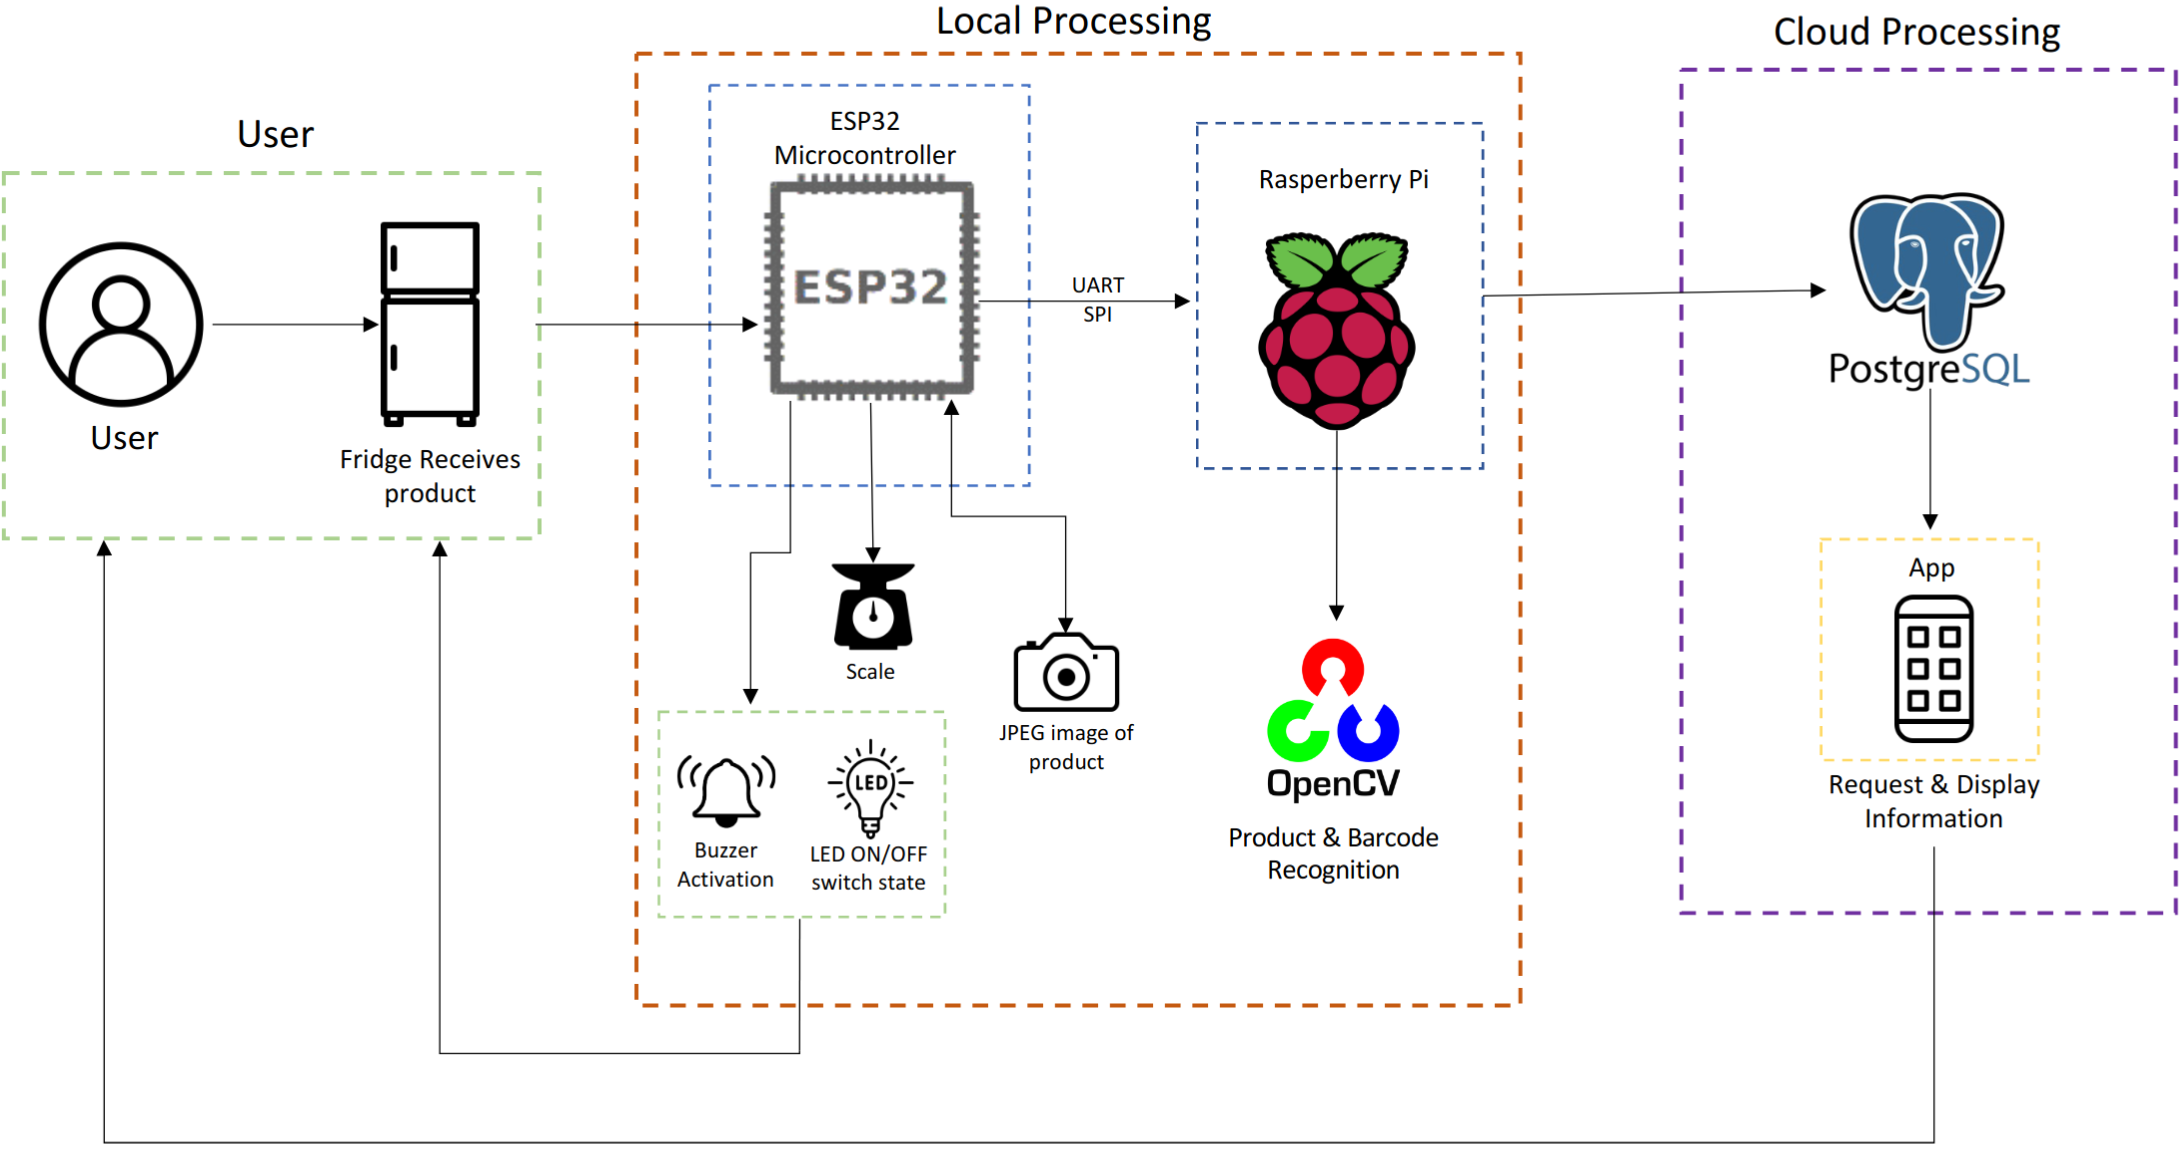
\includegraphics[width=0.75\textwidth]{block-diagram_2.png}
\end{figure} 

The Smart Fridge is designed to be unobtrusive at its core.
In Figure \ref{fig:block_diagram} a system level overview can be seen.
Alongside this diagram, a MoSCoW Table \ref{tab:mscw} was produced to showcase the priority of features.
The heart of the hardware design is the ESP32 microcontroller which interfaces with a pressure sensor,
an OV2640 camera module and HAL effect switches.
The HAL switches detect when the fridge opens and then the OV2640 takes pictures.
The camera will capture several images of the item entering or exiting the fridge.
By measuring pressure, the changes in weight can be registered, helping determine if an item has been removed or added.
Data is then sent to the Raspberry Pi over a serial connection.
A motherboard shall be produced to distribute power to the devices,
as well as connect the sensors to the ESP.
If the door is left open, a buzzer will sound, reminding the user to close the door.  

The Raspberry Pi acts as the bridge between the fridge and the Supabase backend (hosted on AWS).
The image will be run through OpenCV to detect barcodes,
and by maintaining a database of barcodes and associated items we can identify items using the barcodes.
However, for barcode-less products, OpenCV's object detection libraries will be used to identify the item.
Furthermore, Optical Character Recognition (OCR) will be implemented to extract expiry dates.  

The identified product and expiration data will then be sent from the Pi to the PostgreSQL server using the GraphQl API.
The user will be able to view the contents of their fridge from the React App or website,
as well as edit the products currently listed, in case of missing items.
They will also receive notifications if items are going to expire.
By looking at the contents of the fridge, recipes will be suggested, and nutritional information will be provided by plugging into existing APIs[4].  

\begin{table}[H]
    \centering
    \small
    \caption{MoSCoW}
    \label{tab:mscw}
    \begin{tabular}{|l|l|l|l|}
    \hline
    \cellcolor[HTML]{9AFF99}\textbf{Must} &
      \cellcolor[HTML]{FFFC9E}\textbf{Should} &
      \cellcolor[HTML]{FFCE93}\textbf{Could} &
      \cellcolor[HTML]{FD6864}{\color[HTML]{000000} \textbf{Wont}} \\ \hline
    Track inventory with     & Track inventory         &                    &                         \\
    minimal user input       & without user input      &                    &                         \\ \hline
    Track Expiration date &
      Track Expiration Date &
      Track Expiration Date &
      Expired Food Detection \\
                             & with minimal user input & without user input &                         \\ \hline
    Work in cold temperature &                         &                    &                         \\ \hline
    Be a normal fridge       &                         & Generate Shopping  & Suggested Shopping /    \\
    feel seamless            &                         & List               & Automatic Shopping      \\ \hline
                             & Suggest Recipes         &                    &                         \\ \hline
                             & Give Nutritional        & Make Nutritional   & Calorie / Macronutrient \\
                             & Information             & Suggestions        & tracking                \\ \hline
    Website or App           & Website and App         &                    &                         \\ \hline
    \end{tabular}
\end{table}
